\documentclass{report}
\usepackage[T1]{fontenc} % Fontes T1
\usepackage[utf8]{inputenc} % Input UTF8
\usepackage[backend=biber, style=ieee]{biblatex} % para usar bibliografia
\usepackage{csquotes}
\usepackage[portuguese]{babel} %Usar língua portuguesa
\usepackage{blindtext} % Gerar texto automaticamente
\usepackage[printonlyused]{acronym}
\usepackage{hyperref} % para autoref
\usepackage{graphicx}

\bibliography{bibliografia}


\begin{document}
%%
% Definições
%
\def\titulo{Procrastinação}
\def\data{\today}

\def\autores{Alexandre Martins, Tomás Rodrigues }
\def\autorescontactos{(103552) alexandremartins@ua.pt, (104090) tcercarodrigues@ua.pt}
\def\departamento{\ac{deti}}
\def\empresa{Universidade de Aveiro}
\def\logotipo{ua.pdf}
%
%%%%%% CAPA %%%%%%
%
\renewcommand{\contentsname}{Índice}
\begin{titlepage}

\begin{center}
%
\vspace*{50mm}
%
{\Huge \titulo}\\ 
%
\vspace{10mm}
%
{\Large \empresa}\\
%
\vspace{10mm}
%
{\LARGE \autores}\\ 
%
\vspace{30mm}
%
\begin{figure}[h]
\center
\includegraphics{\logotipo}
\end{figure}
%
\vspace{30mm}
\end{center}
%
\begin{flushright}

\end{flushright}
\end{titlepage}

%%  Página de Título %%
\title{%
{\Huge\textbf{\titulo}}\\
{\Large \departamento\\ \empresa}
}
%
\author{%
    \autores \\
    \autorescontactos
}
%
\date{\data}
%
\maketitle

\pagenumbering{roman}

%%%%%% RESUMO %%%%%%
\begin{abstract}

\paragraph{}

Procrastinação  é o ato de atrasar ou adiar desnecessária e voluntariamente algo, apesar do conhecimento que haverá consequências negativas para tal. A palavra originou da palavra latina \textit{procrastinatus}, que evoluiu do prefixo pró, que significa "para a frente", e \textit{crastinus}, que significa "de amanhã". Muitas vezes, é um comportamento humano habitual.
\par
Embora seja tipicamente visto como algo negativo devido ao seu efeito prejudicial sobre a produtividade, estando frequentemente associado a depressão, baixa autoestima, culpa e inadequação, também pode ser considerado uma resposta sábia a certos desafios que podem apresentar resultados arriscados ou negativos ou exigir a espera pela chegada de novas informações.
\par

Cada um dos vários tipos de procrastinação (como académica / não académica ou comportamental / indecisa) têm as suas próprias causas e efeitos subjacentes. A explicação mais proeminente na literatura atual baseia-se na "aversão à tarefa e certos traços de personalidade, como indecisão e distração", como as causas comuns de procrastinação. 
\par
Estudo dos padrões do comportamento dos pombos, por meio da gratificação retardada, sugere que a procrastinação não é exclusiva dos humanos, mas também pode ser observada em alguns outros animais. Quatro em cada cinco aves escolheram a opção mais difícil e complexa, devido à possibilidade de a adiar, ao invés da alternativa que, apesar de mais fácil, implicava que esta fosse começada de imediato.


\end{abstract}

%%%%%% Agradecimentos %%%%%%
% Segundo glisc deveria aparecer após conclusão...
\renewcommand{\abstractname}{Agradecimentos}
\begin{abstract}
\par
Queríamos agradecer aos nossos professores da unidade curricular de Introdução à Engenharia Informática, António Manuel Adrego da Rocha e Óscar Narciso Mortágua Pereira, por nos terem fornecido as ferramentas e conhecimentos necessários para a realização deste projeto, com eles aprendemos como utilizar \textbf{\textit{Code UA}} e os seus beneficios assim como redigir textos em \textbf{\LaTeX}.
\end{abstract}


\tableofcontents
% \listoftables     % descomentar se necessário
% \listoffigures    % descomentar se necessário


%%%%%%%%%%%%%%%%%%%%%%%%%%%%%%%
\clearpage
\pagenumbering{arabic}

%%%%%%%%%%%%%%%%%%%%%%%%%%%%%%%%
\chapter{Introdução}
\label{chap.introducao}

\paragraph{}
Neste relatório será abordado o tema "Procrastinação", comportamento este que tende a surgir aquando um indivíduo se encontra confrontado com algo desagradável ou que pode causar stress como tratar da roupa, estudar ou mesmo interações sociais. É caraterizado pela intensa vontade de adiar uma determinada tarefa, mesmo sabendo que esta terá de ser realizada mais tarde ou mais cedo. Este tema surgiu interesse pelo facto de ser algo com que nos encontrámos com frequência, quer na vida quotidiana assim como estudante.
\par
Irá se tentar perceber no que consiste, como funciona, assim como as suas virtudes e limitações.
\par

Este documento está dividido em 8 capítulos.
\par
Depois desta introdução,
no \autoref{chap.causas},são apresentados 2 subcapitulos com as origens da Procrastinação, \autoref{chap.psicológica} e  \autoref{chap.fisiológica}. No \autoref{chap.saúde} é aborado o ciclo vicioso ente saúde e procrastinação, assim como a influência da personalidade, \autoref{chap.personalidade},  mediadores, \autoref{chap.mediadores}, da genética \autoref{chap.genética} e 5 fatores importantes, \autoref{chap.fatores}. No \autoref{chap.cultura} é abordado o impacto da cultura na procrastinação seguem-se correlações como perfecionismo e o síndrome do estudante no \autoref{chap.Correlações}, \autoref{chap.perfecionismo} e \autoref{chap.adacemico} respetivamente. No \autoref{chap.tipos} temos 2 tipos de procratinadores, relaxado (\autoref{chap.relaxado}) e tenso-nervoso (\autoref{chap.tenso}).
Finalmente, no \autoref{chap.soluçoes} temos sugestões para reduzir a tendência a procratinar seguida do \autoref{chap.conclusao} , onde são apresentadas as conclusões do trabalho.

%-----------------------------------------------------------------


\chapter{Causas}
\label{chap.causas}


\section{Psicológica}
\label{chap.psicológica}
\paragraph{}
As causa psicológicas da procrastinação podem variar muito, mas geralmente provêm de fatores como a ansiedade, baixa auto-estima e uma mentalidade auto-destrutiva. Pensamentos como "ninguém manda em mim" que tornam possível ao indivíduo dar-se ao luxo de ignorar/adiar os seus deveres, outros pensamentos que dão uma urgência em sentir prazer, medo de falhar, incerteza e insegurança contribuem imenso para a realização do ato de procrastinação.

Para o autor David Allen existem duas grandes causas psicológicas de procrastinação no trabalho e no dia a dia. Estas estão relacionadas a problemas de ansiedade e de preguiça emocional. 

O primeiro caso engloba coisas muito pequenas para se preocupar, tarefas "triviais" que são consideradas pelo sujeito como fúteis interrupções que impedem o fluxo das coisas. Vale dizer também que as soluções são subestimadas igualmente pelo sujeito que tende a achar que o impacto destas não é relevante.

O segundo caso contém coisas muito grandes para serem controladas, tarefas temidas pela sua importância ou complexidade, como o exemplo mais famoso e comum, um estudante que teme tanto um exame que adia ao máximo o seu preparo, muita das vezes por pressão, seja esta causada por ele mesmo, por o próprio estabelecimento de ensino, ou até pelos familiares.

\vspace{3mm}


Como já pode ser deduzido, o prazer pode ser considerado um dos grandes culpados pela procrastinação, por este as pessoas preferem evitar emoções negativas atrasando assim tarefas trabalhosas. Normalmente à medida que o fim dos prazos das tarefas adiadas se aproxima os procrastinadores tendem a ficar mais nervosos e ansiosos e assim finalmente acabando por realizar as suas tarefas, no entanto estas são concluídas na forma mais stressante e nociva para a saúde mental do indivíduo.

\vspace{10mm}

Para além da mentalidade mencionada acima ainda existem estratégias orientadas pela emoção utilizadas pelos procrastinadores.
\begin{itemize}
    \item Prevenção: Evitar o local ou situação onde a tarefa ocorre.
    \item Negação e trivialização: Fingir que o comportamento procrastinatório não é realmente procrastinador, mas sim uma tarefa que é mais importante do que a evitada, ou que a tarefa essencial que deve ser realizada não é de importância imediata.
    \item Distração: envolver-se ou imergir em outros comportamentos ou ações para prevenir a consciência da tarefa.
    \item Contrafatualidade descendente: Comparação das consequências do comportamento procrastinatório de uma pessoa com as piores situações de outras pessoas.
    \item Valorização: apontar com satisfação para o que se alcançou enquanto deveria estar a fazer outra coisa.
    \item Culpar: Atribuições delirantes a fatores externos, como racionalizar que a procrastinação se deve a forças externas além do controle.
    \item Caçoar: usar o humor para validar a procrastinação.
\end{itemize}

Medidas de resolução de tarefas ou problemas são desgastantes do ponto de vista de um procrastinador. Se tais medidas forem adotadas, é menos provável que o procrastinador permaneça com tais comportamentos nocivos. No entanto, buscar tais medidas requer uma mudança ativa de comportamento ou situação para prevenir e minimizar a recorrência da procrastinação.



\section{Fisiológica}
\label{chap.fisiológica}

Investigações sobre as raízes fisiológicas da procrastinação têm se focado no papel do córtex pré-frontal, na área do cérebro que é responsável pelas funções cerebrais executivas, como controlo de impulsos, atenção e planejamento. Isso é consistente com a noção de que a procrastinação está fortemente relacionada a essas funções, ou à falta delas. O córtex pré-frontal também atua como um filtro, diminuindo os estímulos de distração de outras regiões do cérebro. Danos ou baixa ativação nesta área podem reduzir a capacidade de evitar desvios, o que resulta em pior organização, perda de atenção e aumento da procrastinação. Isso é semelhante à função do lobo pré-frontal no transtorno de defice de atenção, onde é comumente subutilizado. 



\chapter{Saúde}
\label{chap.saúde}


\paragraph{}
Até um certo grau, é normal procrastinar e pode ser considerado uma forma útil de organizar tarefas, destacando e dando prioridade às de verdadeira importância. No entanto, a procrastinação excessiva pode tornar-se um problema, impedindo o funcionamento saudável da vida quotidiana. Esta ocorre frequentemente, em simultâneo, com problemas de saúde, stress, ansiedade, sentimentos de culpa, bem como perda de produtividade pessoal e desaprovação social por não cumprir responsabilidades ou compromissos. Juntos, estes sentimentos podem promover mais procrastinação e, para alguns indivíduos, a procrastinação torna-se quase crônica. Estes individuos podem ter dificuldade em procurar apoio devido à própria procrastinação, mas também aos estigmas sociais e à crença de que a aversão à tarefa é causada pela preguiça, falta de força de vontade ou baixa ambição. Em alguns casos, a procrastinação problemática pode ser um sinal de algum distúrbio psicológico subjacente. Criando então um ciclo vicioso de  improdutividade.
%%%%%
Em termos de procrastinação, a via comportamental indireta pode ser a rota mais importante para a compreensão dos possíveis efeitos negativos da procrastinação sobre a saúde. Isso não quer dizer que o stress experimentado pelos procrastinadores não envolva mudanças no funcionamento do sistema imunológico que possam comprometer a saúde. Na verdade, a associação entre estados de humor negativos e procrastinação está bem estabelecida, e essas mudanças afetivas são conhecidas por impactar negativamente o funcionamento do sistema imunológico. Porém, de acordo com Milgram (1991), a perturbação emocional vivida pelos procrastinadores é resultado da sequência comportamental de adiamento, portanto, estes estados de humor negativos são, em grande parte, o resultado das manifestações comportamentais da procrastinação, e não a causa do comportamento dilatório.

Ao contrário de outras construções de personalidade, como o padrão comportamental do Tipo A, que pode estar ligado à saúde principalmente por meio de vias reativas ou diretas com o comportamento como uma via secundária, a procrastinação pode ser considerada como influenciando a saúde principalmente por meio indireto meios comportamentais. Consequentemente, argumentamos que a tendência dos procrastinadores de atrasar tarefas é a causa proximal de seus estados de humor negativos e aumento do stress, em oposição a uma propensão fisiológica inata para reagir a situações de forma stressante, que pode predispô-los a problemas de saúde.

Esta conceituação de procrastinação como um estilo de comportamento que afeta a saúde física encaixa-se em uma das três principais rotas sugeridas por Suls e Rittenhouse (1990) para explicar a relação entre personalidade e aumento do risco de doença. De acordo com o “modelo de personalidade como preditor de comportamento perigoso”, certos perfis de personalidade levam à criação ou escolha de situações que provocam reatividade, criam stress desnecessário, promovem comportamentos não saudáveis ou impedem comportamentos preventivos. Além disso, é uma combinação de hábitos prejudiciais à saúde, como dieta inadequada, falta de atividade, exposição a fatores de stress e não conformidade com regimes médicos, que é a chave para prever o risco de doença, e não a frequência ou magnitude de qualquer comportamento.

\vspace{5mm}
\begin{figure}[h]
\center
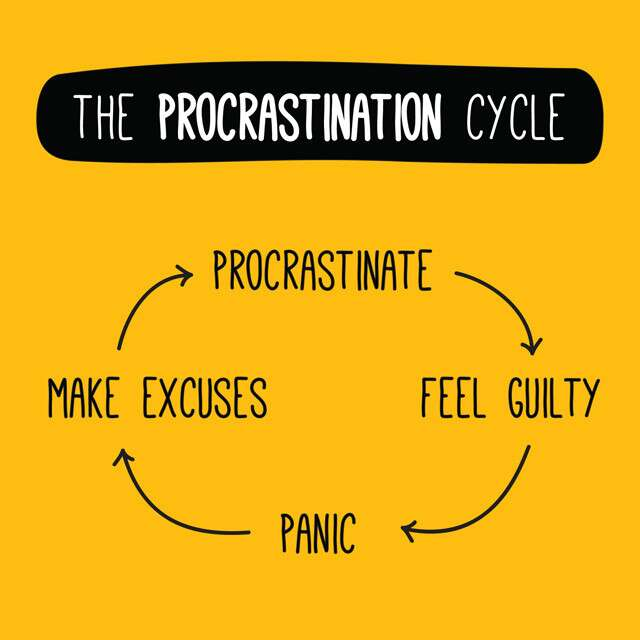
\includegraphics[width=7cm, height=4cm]{ligma.jpg}
\caption{Ciclo vicioso da procrastinação com saúde}
\end{figure}

\section{Personalidade}
\label{chap.personalidade}
\paragraph{}
Pesquisas teóricas e empíricas atuais sobre a relação entre personalidade e saúde oferecem algum suporte para as associações entre procrastinação, stress e saúde sugeridas por Tice e Baumeister (1997). As investigações dos efeitos do stress no sistema imunológico têm sido uma área frutífera de pesquisa em psiconeuroimunologia humana (PNI) por mais de uma década. Este crescente corpo de literatura sugere que os eventos stressantes da vida estão relacionados ao aumento da vulnerabilidade a condições infecciosas, como o constipação, bem como mau estado de saúde.

Sergerstrom (2000) propõe que a relação personalidade-sistema imunológico pode ser explicada por vários mediadores psicossociais, incluindo o impacto do stress, conforme sugerido pela pesquisa do PNI. Especificamente, a quantidade ou qualidade do stress experimentado pode ser uma função da personalidade e esse stress, por sua vez, afeta o sistema imunológico. Como sugere Sergerstrom, essa relação é complexa, com a personalidade implicada tanto na exposição a atividades stressantes quanto na subsequente reatividade a esses eventos stressantes. Além disso, outros fatores psicossociais e comportamentais podem influenciar o funcionamento imunológico e as alterações subsequentes no estado de saúde, seja interagindo com ou independentemente de eventos stressantes.

Da mesma forma, Friedman (2000) afirma que existem dois tipos gerais de mecanismos que medeiam a relação entre personalidade e saúde: (1) padrões de reação psicofisiológica que incluem mudanças na função imunológica devido ao stress; e (2) comportamentos de saúde. Outras formulações de como a personalidade afeta os resultados de saúde referem-se a essas duas rotas como vias diretas e indiretas. A primeira se refere à reatividade psicofisiológica associada à ativação da resposta ao stress e suas vias neuroendócrinas associadas, enquanto a última reflete as vias comportamentais e a interação da personalidade com o meio ambiente.

\section{5 fatores importantes}
\label{chap.fatores}
\paragraph{}
Embora a relação entre procrastinação e comportamentos de saúde não tenha sido investigada formalmente, pesquisas anteriores sugerem que certas dimensões de personalidade de ordem superior podem estar associadas a uma variedade de comportamentos relacionados à saúde. Muitas dessas pesquisas empregaram o modelo de cinco fatores da personalidade como uma estrutura para compreender a relação entre a personalidade e os padrões de comportamento de saúde. Dois preditores consistentes de comportamentos de saúde que emergiram desta pesquisa são conscienciosidade e neuroticismo.

Conscienciosidade, a tendência para a persistência, direcionamento ao objetivo e organização, foi encontrada em um estudo para ser substancialmente relacionada a taxas mais altas de comportamentos de bem-estar (por exemplo, dieta adequada, sono e exercícios), controle de acidentes (por exemplo, consertar riscos domésticos) e menor taxas de assunção de riscos no trânsito e de riscos relacionados a substâncias. Outros estudos associaram a baixa conscienciosidade a níveis mais baixos de comportamentos promotores da saúde, como exercícios, e níveis mais altos de comportamentos não saudáveis, como fumar e beber em excesso.

O neuroticismo, uma disposição para vivenciar fortes emoções negativas e vulnerabilidade ao stress, também pode afetar o sistema imunológico por meio de uma via de comportamento de saúde (Sergerstrom, 2000). A pesquisa sugere que tanto o aumento das práticas de saúde prejudiciais quanto a redução de comportamentos positivos de saúde estão associados a este importante traço de personalidade (Booth-Kewley e Vickers, 1994, Lemos-Giraldez e Fidalgo-Aliste, 1997, Mechanic e Cleary, 1980, Vingerhoets et al., 1990).

Investigações recentes da relação entre a procrastinação e o modelo de cinco fatores identificaram a consciência e neuroticismo como os dois principais fatores associados à procrastinação. Esses estudos indicam que a conscienciosidade está altamente e negativamente relacionada à procrastinação e contribui significativamente para a variância nos valores de procrastinação, especialmente a procrastinação para evitar a tarefa. No entanto, quando comparada à conscienciosidade, a procrastinação é o melhor preditor de comportamento dilatório específico de traço. O neuroticismo, entretanto, está positivamente associado à procrastinação e está principalmente relacionado à tentativa direcionada para um objetivo e à procrastinação decisória.

\section{Mediadores}
\label{chap.mediadores}
\paragraph{}
A conexão entre procrastinação e conscienciosidade (e em menor extensão neuroticismo) e o impacto desses fatores de personalidade de ordem superior nos comportamentos de saúde fornecem uma explicação plausível para a mediação dos efeitos da procrastinação na saúde. Comportamentos de bem-estar são comportamentos de promoção ou manutenção da saúde (por exemplo, exercícios, dieta adequada) que podem ajudar a atenuar os efeitos do stress, bem como melhorar os estados de saúde. No entanto, esses comportamentos de saúde são frequentemente vistos como desafiadores e/ou desagradáveis. Dado que a aversividade à tarefa está relacionada à procrastinação é provável que os procrastinadores poçam “adiar” muitos comportamentos de saúde como comportamentos de bem-estar, que são vistos como desagradáveis.

A procrastinação também pode estar relacionada a comportamentos terapêuticos de saúde importantes, como a procura de tratamento. Atraso na procura de tratamento é um comportamento dilatório específico da saúde, frequentemente referido como atraso do paciente e definido como o período de tempo entre a primeira percepção do indivíduo de um sintoma e o momento da consulta médica. O atraso na procura de tratamento por problemas de saúde tem sido conceituado como um processo de várias etapas composto por atrasos na avaliação dos sintomas como sinais de doença (atraso na avaliação), na decisão de procurar tratamento (atraso na doença), agindo sobre esta decisão (atraso comportamental ), e até ser atendido por um profissional médico (atraso no agendamento). É possível que a procrastinação, uma variável da personalidade que afeta diretamente o comportamento, possa influenciar o estágio de retardo comportamental da busca por tratamento.


Comportamentos de bem-estar, como exercícios e dieta adequada, são bem conhecidos por serem afetados pelos níveis de Stress, especialmente em populações de estudantes. Dada a associação negativa entre procrastinação e conscienciosidade, e a relação positiva entre conscienciosidade e comportamentos de saúde positivos, esperava-se que a procrastinação estivesse associada a menos comportamentos de bem-estar. Assim, esperava-se que os comportamentos de bem-estar estivessem associados a alto stress e problemas de saúde (ver Fig. 3.2).

\vspace{90mm}
\begin{figure}[h]
\center
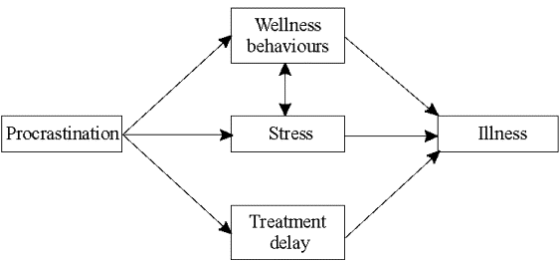
\includegraphics[width=9cm, height=4cm]{uwu.png}
\caption{Relação da procrastinação com saúde}
\end{figure}



\section{Genética}
\label{chap.genética}
\paragraph{}

Num estudo americano de 2014 cujo foco era procrastinação e impulsividade em pares de gêmeos fraternos e idênticos, ambas as características foram consideradas "moderadamente hereditárias". As duas características não
foram separáveis no nível genético (r {\tiny genetic} = 1.0), o que significa que nenhuma influência genética única de qualquer uma das características foi encontrada. Os autores confirmaram três construtos desenvolvidos a partir da hipótese evolutiva de que a procrastinação surgiu como um subproduto da impulsividade: 
\begin{itemize}
  \item A procrastinação é hereditária;
  \item As duas características compartilham uma variação genética considerável;
  \item A capacidade de gerenciamento de metas é uma componente importante desta variação compartilhada.
\end{itemize}


\chapter{Cultura}
\label{chap.cultura}
\paragraph{}
De acordo com Holly McGregor e Andrew Elliot em 2002 e Christopher Wolters em 2003, procratinação academica entre estudantes encontra-se correlacionada com \ac{pao}, isto foca-se em evitar uma tarefa devido à crença que o indivíduo não é bom o suficiente para a realizar com sucesso, que é 1 fator de 4 no total, do modelo de orientação para o desempenho. Andrew Elliot e Judith Harackiewicz em 1996 mostraram que alunos com \ac{pao} tendem a preocupar-se mais com as comparações com os seus colegas. Estes alunos procrastinaram como resultado de não quererem parecer incompetentes ou para evitar demonstrar uma falta de habilidade e adotar uma aparência de competência em frente aos seus colegas.

Gregory Arief Liem e Youyan Nie, em 2008, descobriram que as características culturais demonstraram ter uma influência direta na \ac{pao} porque estão diretamente alinhadas com os valores e crenças da maioria dos alunos. A meta-análise de Sonja Dekker e Ronald Fischer, em 2008, em treze sociedades diferentes revelou que os alunos de culturas ocidentais tendem a ser mais motivados pela \ac{mao}, isto é, a organização de tarefas de acordo com a competência do individuo perante as tarefas, porque o grau de valor de incentivo para o desempenho individual reflete fortemente os valores da cultura ocidental. Por contraste, descobriu-se que a maioria dos alunos de culturas orientais focam-se em \ac{pao}. Estes, frequentemente, esforçam-se para manter uma imagem positiva das suas habilidades, que exibem à frente dos colegas. Para além disto, Hazel Rose Markus e Shinobu Kitayama, 1991, mostraram que em culturas não ocidentais, ao invés de destacar os seus feitos, as pessoas tendem a ser motivadas a se tornarem parte de vários relacionamentos interpessoais e de se encaixar naqueles que lhes são relevantes.

A pesquisa de Sushila Niles, 1998, com estudantes australianos e estudantes do Sri Lanka confirmou essas diferenças, revelando que os estudantes australianos frequentemente iam em busca de objetivos mais individuais, enquanto os estudantes do Sri Lanka geralmente desejavam objetivos mais colaborativos e sociais. Vários estudos de Kuo-Shu Yang e An-Bang Yu, 1987, 1988 e 1990, indicaram que o desempenho individual entre a maioria dos alunos chineses e japoneses era medido pelo cumprimento de suas obrigações e responsabilidades para com sua rede familiar, ao invés de realizações individuais. Yang e Yu, 1987, também mostraram que o coletivismo e o confucionismo são motivadores muito fortes para realizações em muitas culturas não ocidentais por causa da sua ênfase na cooperação na unidade familiar e na comunidade. Guiado por estes valores culturais, acredita-se que o indivíduo tende a sentir,intuitivamente, um grau de pressão social, "Peer Pressure", sendo esta a causa do foco em objetivos que beneficiam a comunidade ao invez do indiviuo.
\chapter{Correlações}
\label{chap.Correlações}

\section{Perfecionismo}
\label{chap.perfecionismo}
\paragraph{}

O psicólogo William J. Knaus estimou que mais de 90\% dos estudantes universitários procrastinam. Desses alunos, 25\% são procrastinadores crônicos, que normalmente acabam por abandonar o ensino superior.

Tradicionalmente, a procrastinação é muitas vezes associada ao perfeccionismo, dando a tendência de avaliar negativamente o resultado dos próprios esforços. Existe também um receio imenso à avaliação das próprias habilidades por terceiros, uma "autoconsciência social" elevada e ansiedade, mau humor recorrente e "\textit{workaholism}". 

Contudo, os perfeccionistas adaptativos, "\textit{perfeccionismo egossintônico}", são menos propensos a procrastinar do que os não prefeccionistas, enquanto os perfeccionistas desadaptativos que vêm o seu prefeccionismo como algo negativo, perfeccionismo egodistônico, procrastinavam imenso e sofriam de ansiedade.
    
\section{Acadêmico}
\label{chap.adacemico}

\paragraph{} 
A procrastinação é sem dúvida um aspeto recorrente na vida académica de imensos estudantes, onde estes lidam constantemente com prazos, seja para exames, seja para projetos.

A procrastinação é enfrentada por estes geralmente por vários motivos, má gestão de tempo, stress, falta de técnicas de estudo, ou porque estes sentem-se sobrecarregados com trabalho. Estes ainda podem encarar este problema por razões clínicas como défice de atenção ou dislexia.

Não é conhecido o quão comum um caso severo de procrastinação por causa clínica pode passar escondido quando a pessoa se encontra num ambiente académico, pois pode ser meramente catergorizada como "procrastinação acadêmica".



\chapter{Tipos de procrastinadores}
\label{chap.tipos}

\paragraph{} 
A reação do indivíduo quanto ao seu acto de procrastinação pode variar perdominantemente entre dois tipos. Existem os que reagem de uma forma mais relaxada fugindo das suas responsabilidades e depois temos os que são esmagados pela pressão.
\section{Tipo relaxado}
\label{chap.relaxado}

\paragraph{}
Os procrastinadores do tipo relaxado vêm as suas responsabilidades de forma negativa, que nem os demais, porém estes fogem destas direcionando a própria energia para outras tarefas. É comum, por exemplo, para um estudante procrastinador do tipo relaxado, abandonar os seus trabalhos e projetos, mas não a sua vida social assim continuando a frequentar bares e festas deixando de lado os seus deveres. Esse tipo de procrastinação é tido como uma forma de negação. O procrastinador evita situações que lhe poçam causar desprazer, e, em vez delas, participa de situações mais prazerosas.  

Esses procrastinadores se recusam a renunciar ao princípio do prazer, em vez de sacrificarem-se no \textit{princípio da realidade}. Eles podem aparentar não estar preocupados com o trabalho e com prazos, mas isso é simplesmente uma forma de evasão.

\section {Tipo tenso-nervoso}

\paragraph{} O procrastinador do tipo tenso-nervoso normalmente é dominado pela pressão, esta é esmagadora quando trata-se de tempo, assim, sem mínima certeza dos seus objetivos e junto de imensos outros sentimantos negativos e prejorativos para o seu bem estar e saúde mental. Sentindo que lhes falta a habilidade ou foco para completar os seus deveres, estes dizem a si mesmos que precisam de se acalmar e relaxar, e que é melhor ter calma e adiar para o dia seguinte, ou para quando este se sentir melhor, por exemplo.

A tarefa ser adiada para o procrastinador "relaxar" é uma ação geralmente temporária e inefetiva, levando a este maior quantidade de stress conforme o prazo vai se esgotando. À medida que os prazos se aproximam a pessoa vai se sentindo cada vez mais culpada, desgastada e apreensiva. Esse comportamento tende a virar um ciclo de fracasso e atrasos, enquanto as tarefas e deveres são constantemente adiados e deixados de lado para uma data mais confortável. Isto também acarreta efeitos debilitantes e bem negativos para a vida pessoal e social do sujeito.

Como procrastinadores deste tipo são incertos quanto aos seus objetivos e constantemente dominados pela culpa, estes tendem a sentir-se desconfortáveis perto daqueles que não sofrem com tais problemas, assim causando até depressão. Logo, procrastinadores tensos-nervosos geralmente recolhem-se da vida social, evitando contacto até mesmo com amigos próximos.


\label{chap.tenso}

%more some more%


\chapter{Soluções}
\label{chap.soluçoes}
\paragraph{}

Comportamentos e práticas que reduzem a procrastinação:
\begin{itemize}
  \item Realização dos hábitos e pensamentos que levam à procrastinação;
  
  \item Pedir ajuda a familiares, amigos e profissionais para problemas autodestrutivos, como medo, ansiedade, dificuldade de concentração, má administração do tempo, indecisão e perfecionismo;
  
  \item Avaliação justa de objetivos pessoais, forças, fraquezas e prioridades;

  \item Estabelecer metas realistas e associar ligações positivas entre as tarefas e as metas concretas estabelecidas anteriormente;

  \item Estruturação e organização das atividades diárias;

  \item Mudar de ambiente, reduzindo a sensação de aborrecimento, que se estabelece após algumas horas. Locais calmos como bibliotecas e salas de estudo têm tendência a ser os mais utilizados mas também há quem prefira ambientes com maior movimento como cafés e parques;
  
  \item    Disciplinar-se para definir prioridades;

  \item "Positive Reinforcement" - Ser recompensado após cada tarefa com tarefas agradáveis e não viciantes como redes sociais. Alguns exemplos são caminhadas, socializar e brincar com animais;
  
  \item Separar tarefas em pequenos blocos, em vez de tentar problemas inteiros de uma vez;

  \item Para evitar recaídas, é importante reforçar metas pré-estabelecidas com base nas necessidades atuais e ser recompensado de forma balançada com a dificuldade das tarefas realizadas.
  
 \end{itemize}




\chapter{Conclusão}
\label{chap.conclusao}
\paragraph{}

A procrastinação é um problema que afeta grande parte da população, sobretudo estudantes, e como visto anteriormente esta possui várias causas quer de cariz psicológico ou fisiológico, variando entre pensamentos danosos para a eficiência e bem-estar do sujeito até "reais" problemas psicológicos como dislexia e défice de atenção. 

Independentemente da causa, procrastinação é surpreendentemente um assunto extremamente sério pois não é apenas algo que nos afaste e bloqueia os caminhos até os nossos objetivos, mas também pode destruir o nosso psicológico ou impedir que realizemos a procura da solução para outros problemas.



\chapter*{Contribuições dos autores}
\paragraph{}

 O trabalho foi feito presencialmente na totalidade pelo que cada um contribuiu um pouco para todas as partes, no entanto as tarefas alocadas a cada membro foram, para o Alexandre Martins introdução, saúde, cultura e soluções sendo que o Tomás Rodrigues ficou com as restantes, isto é causas, correlações, tipos de procrastinadores, conclusão e como foi feito presencialmente não sentimos necessidade de fazer ambos git push pelo que ele tratou também desta parte.

 Desta forma concordamos que cada um merece 50\%.

%%%%%%%%%%%%%%%%%%%%%%%%%%%%%%%%%
\chapter*{Acrónimos}
\begin{acronym}
\acro{ua}[UA]{Universidade de Aveiro}
\acro{lei}[LEI]{Licenciatura em Engenharia Informática}
\acro{deti}[DETI]{Departamento de Eletrónica, Telecomunicações e Informática}
\acro{glisc}[GLISC]{Grey Literature International Steering Committee}
\acro{pao}[PAO]{Performance-Avoidance Orientated}
\acro{mao}[MAO]{Mastery-Approach Orientation}
\end{acronym}


%%%%%%%%%%%%%%%%%%%%%%%%%%%%%%%%%
\chapter*{Bibliografia}
\begin{flushleft}
\begin{itemize}
\paragraph{}
\item "Why Do We Procrastinate?",
https://www.youtube.com/watch?v=pKyHX0zqynk
\paragraph{}
\item"What Is Procrastination?",
https://www.verywellmind.com/the-psychology-of-procrastination-2795944
\paragraph{}
\item"Procrastination",
https://en.wikipedia.org/wiki/Procrastination
\paragraph{}
\item"Procrastinação",
https://pt.wikipedia.org/wiki/Procrastina\%C3\%A7\%C3\%A3o
\paragraph{}
\item"Conheça as 4 CAUSAS REAIS da PROCRASTINAÇÃO"
https://youtu.be/CkMAE5Jav20
 \end{itemize}

\end{flushleft}


\printbibliography

\end{document}
